%% Author_tex.tex
%% V1.0
%% 2012/13/12
%% developed by Techset
%%
%% This file describes the coding for rsproca.cls

\documentclass[openacc]{rsproca_new}%%%%where rsproca is the template name
\usepackage{subcaption}
%%%% *** Do not adjust lengths that control margins, column widths, etc. ***

%%%%%%%%%%% Defining Enunciations  %%%%%%%%%%%
\newtheorem{theorem}{\bf Theorem}[section]
\newtheorem{condition}{\bf Condition}[section]
\newtheorem{corollary}{\bf Corollary}[section]
%%%%%%%%%%%%%%%%%%%%%%%%%%%%%%%%%%%%%%%%%%%%%%%

%%%%% Please insert respective article type here %%%%
\titlehead{Research}

\begin{document}

%%%% Article title to be placed here
\title{Inferring the shape of an object inside of a draining tank}

\author{%%%% Author details
Gbenga Fabusola$^{1}$, 
Cory M. Simon$^{1}$
}

%%%%%%%%% Insert author address here
\address{$^{1}$School of Chemical, Biological, and Environmental Engineering. Oregon State University. Corvallis, OR, USA.
% $^{2}$Second author address\\
}

%%%% Subject entries to be placed here %%%%
\subject{applied mathematics, chemical engineering}

%%%% Keyword entries to be placed here %%%%
\keywords{inverse problems, Bayesian statistical inversion, Torricelli's law}

%%%% Insert corresponding author and its email address}
\corres{Cory M. Simon\\
\email{cory.simon@oregonstate.edu}}

%%%% Abstract text to be placed here %%%%%%%%%%%%
\begin{abstract}

\absbreak % unclear why this is needed
\end{abstract}
%%%%%%%%%%%%%%%%%%%%%%%%%%%

\rsbreak

%%%%%%%%%% Insert the texts which can accomdate on firstpage in the tag "fmtext" %%%%%

\section{Introduction}
Throughout engineering and the applied sciences, we encounter a liquid-holding tank that is draining via gravity-driven flow through a small orifice.
Mathematical models of the dynamics of the liquid level in a draining tank are useful for designing the geometry of the tank and orifice, predicting the emptying time, forecasting the outlet flow rate, controlling the liquid level via an inlet stream, and inferring the liquid level from the outlet flow rate.

Interestingly, ancient societies (e.g. ancient Greece) exploited the predictable dynamics of the water level in a draining tank to measure and display the passage of time.
Specifically, the water clock, or clepsydra (Greek for ''water thief''), of the outflow design consisted of an open-top container, filled with water at some reference time, with a small orifice for outflow near its bottom.
As the clepsydra drained, the elapsed time was visually indicated by the liquid level with respect to graduated markings on the inside of the container. \cite{bedini1962compartmented,hwang2021historical,ritner2016oriental,hejun1987research,schomberg2018karnak,mills1982newton}
E.g. the Karnak clepsydra from $\sim$1300 BC \cite{schomberg2018karnak} was an inverted truncated cone. Notably, this geometry does not provide a constant rate of decrease in the liquid level; perhaps, though, its wider top was intended to compensate for faster outflow at higher liquid levels.

%Draining tanks have been studied since ancient times, as evidenced by water clocks in ancient Egypt, Greece, India, and China.
%The water clock, or clepsydra (Greek for ''water thief''), of the outflow design consisted of an open-top container, filled with water at some reference time, with a small orifice for outflow near its bottom.

%The geometry of an ideal clepsydra would produce a constant rate of decrease in the liquid level. However, the geometry of e.g. the preserved Karnak clepsydra from $\sim$1300 BC \cite{schomberg2018karnak}, an inverted truncated cone, does not. Though, perhaps, its wider top was intended to compensate for the faster outflow when the liquid level is higher.

Italian physicist and mathematician Evangelista Torricelli (1608-1647) made a fundamental observation for mathematical modeling the liquid level in a tank draining via gravity-driven flow through a small orifice: the velocity $v$ at which liquid flows out of the orifice is proportional to the square root of the height of liquid above the orifice, $\Delta h$, i.e. $v\propto \sqrt{\Delta h}$ \cite{mills1982newton}. Today, we recover Torricelli's observation from Daniel Bernoulli's (1700–1782) equation, a mechanical energy balance applied to the steady, plug flow of an incompressible, inviscid fluid through the orifice, with frictional forces neglected. This gives what we today refer to as \emph{Torricelli's law}: $v=\sqrt{2 g \Delta h}$, with $g$ the acceleration due to gravity. \cite{d2021torricelli}

A mass balance and Torricelli's law give a first-order, [generally] nonlinear differential equation describing the liquid level over time in a tank draining of liquid via gravity-driven flow through a small orifice \cite{groetsch1993inverse,seborg2016process}.
The geometry of the tank affects the dynamics of the liquid level through its cross-sectional area (parallel to the ground) as a function of height.
The cross-sectional area of the orifice affects the volumetric flow rate out of the tank.
% TODO: a name for cross-sectional area parallel to the ground?
For agreement with the experimentally measured liquid level in a draining tank over time \cite{de2000pin,blasone2015discharge,wadhwa2021study,liu2008drainage}, a discharge coefficient is introduced into the model as a `fudge factor' to
% Specifically, we model the outlet flow rate as $c a_o \sqrt{2 g \Delta h}$. 
% The discharge coefficient $c$
account for frictional losses across the orifice, non-uniformity of the velocity profile, and a smaller cross-sectional area of the liquid jet than the orifice (vena contracta).
%  and (ii) depends on the rheology of the fluid and the geometry of the orifice. 
\cite{teoman2022discharge,hicks2014determining,blasone2015discharge}

% Note, Torricelli's law combined with kinematic equations on a packet of fluid ejected from the orifice of the tank give the trajectory of the liquid jet, too \cite{groetsch1999inverse}.

A draining tank is an intuitive, relatable physical system to mathematically model in an undergraduate course. 
More, experiments in the classroom to collect data to validate the model of the liquid level over time are accessible and illustrate the effectiveness of mathematical models.
\cite{farmer1992physical,driver1998torricelli,brady2009siphons,rother2024modelling,paldy1963apparatus,ivanov2014testing,williams2021vessel,pavesi2019investigating,planinvsivc2011holes,saleta2005experimental,lopac2015water}
Draining tanks provide undergraduate-friendly inverse problems \cite{groetsch1993inverse,neto2012introduction,tarantola2005inverse} as well, such as inferring (i) the liquid level in the tank from the range of the liquid jet and (ii) the shape of the tank from the liquid level over time \cite{groetsch1993inverse,groetsch1999inverse}. 
An inverse problem pertaining to the outflow clepsydra is: what container shape gives a constant rate of decrease in the liquid level as it drains?
(Using a differential equation model for the liquid level, such a clepsydra may be obtained via a solid of revolution about the vertical axis such that the radius scales with the quartic root of the height. \cite{mills1982newton,d2021torricelli})


\section{Experimental setup}
In our experimental setup, we (1) fill a small, open-top, plastic tank with water, to an initial level $h_0$ [cm], then (2) at time $t:=0$ [s], allow the water to drain out through a small orifice in the side of the tank, near its bottom. We use a liquid level strip to measure the water level in the tank over time, giving time series data $\{(t_i, h_i)\}$. The tank may or may not have a heavy, solid, stationary object inside of it, displacing water and thus affecting the dynamics of emptying. Fig.~\ref{fig:photo_of_tank} shows a photo of our experimental setup (without an object inside of it).

Ultimately, we conduct a set of three experiments. The first two experiments concern the tank without the object, for the purpose of gathering data to calibrate then test a dynamic mathematical model of the liquid level in the tank. The third experiment concerns the tank with an object inside of it, for the purpose of indirectly gathering data about then inferring the shape of the object.

\begin{figure}[h!]
\begin{center}
	% \includegraphics[width=0.3\textwidth]{../tank_geometry/photo_of_tank.png}
	\caption{\textbf{Experimental setup.}}
	\label{fig:photo_of_tank}
\end{center}
\end{figure}

\paragraph{The tank geometry.} The water-holding tank is approximately an inverted, right, truncated cone with a rounded rectangle as its base. The cross-sectional area [parallel to the ground] of the tank as a function of height $h$ [cm] from its bottom base is:
\begin{equation}
	a_t(h) = \frac{h}{H}a_1 + \left(1-\frac{h}{H}\right) a_0,
\end{equation}
with $H$ [cm] the height of the tank and $a_0$ [cm$^2$] and $a_1$ [cm$^2$] the area of the rounded rectangle forming the bottom and top, respectively, base of the tank.
The top of the tank is open to the atmosphere. 

\paragraph{The small orifice in the side of the tank.} The tank has a small, circular hole of radius $r_o$ [cm] in its side---a small height $h_o$ [cm] from the bottom base.
Thus, when the liquid level in the tank is larger than $h_o$, water flows out of this small orifice.
(When drilling the hole, we held the drill bit parallel to the floor.) 

\paragraph{The object [possibly] inside the tank.} We may place a heavy (denser than water), solid object inside the tank. Because the object is solid, it displaces water while in the tank. Because this object is heavy, it remains at rest, at the bottom of the tank, throughout the experiment. Let $a^\prime(h)$ be the cross-sectional [parallel to the floor] area of this object as a function of height $h$.

\paragraph{The liquid level sensor.} We place a liquid level strip vertically inside the tank to measure the water level in the tank over time. The liquid level sensor communicates with an Arduino microcontroller, allowing us to automatically collect the time series data and write it to a file. The liquid level strip functions by virtue of water coming into contact with it and changing the electrical resistance. 
We constructed a calibration curve to map the level sensor reading to the liquid level in the tank, in units of centimeters. 
Note, in our modeling below, we will neglect the volume of liquid displaced by the level strip.

\section{The forward and measurement models}
The \emph{forward model} provides a prediction of the liquid level $h(t)$ [m] in our draining tank over time $t$ [s], \emph{given} the shape of the tank $a(h)$, the shape of the object inside our tank $a^\prime(h)$, the circular orifice radius $r_o$ and height $h_o$, the discharge coefficient $c$, and the initial liquid level $h_0$. 
Coupled with a probabilistic \emph{measurement model} describing the noise in our liquid level sensor, the forward model allows us to compute the \emph{likelihood function}. The likelihood function specifies the probability of observing a time series data set $\{(t_i, h_i)\}$ from our experiment conditioned upon [proposed] functions/values of $a(h)$, $a^\prime(h)$, $r_o$, $h_o$, $c$, and $h_0$. Thus, when these quantities are uncertain/unknown, the likelihood function score the support that the data $\{(t_i, h_i)\}$ lend for them.

Now, suppose we fill the tank to an initial liquid height $h_0 \leq H$ [m] at time $t=0$ [s] then allow it drain through the orifice without further input of liquid. We wish to model the height of liquid in the tank as a function of time, $h=h(t)$, with $t$ [s] time. 

\begin{align}
& [a_t(h)-a^\prime(h)]\frac{dh}{dt}= -c \pi r_o^2 \sqrt{2g (h(t)-h_o)}, \,\,\, t \geq 0 \\
& h(0)=h_0.
\end{align}

\section{Results}
\subsection{Bayesian calibration of the dynamic model of the liquid level}

\subsection{Bayesian inference of the shape of an object inside the tank}

\section{Conclusions and Discussion}

\section{Methods}

\subsection{Details of the forward model}
\paragraph{Torricelli's law.} Given the height of water in the tank is $h$ [cm], we model the velocity $v$ [cm/s] of the jet of water flowing out of the orifice of the tank with Torricelli's law \cite{d2021torricelli}:
\begin{equation}
	v(h)=  \sqrt{2 g(h-h_o)}, \label{eq:Toricelli}
\end{equation} where $g$ [cm/s$^2$] is the acceleration due to gravity. 
Fundamentally, the outflow is driven by gravity exerting a force on the water above the orifice, which creates a hydrostatic pressure in the water at the entrance of the orifice. 
Torricelli's law follows from Bernoulli's equation \cite{welty2020fundamentals}, a mechanical energy balance on the flow through the orifice, treating (i) the flow as steady, plug, and friction-lossless and (ii) the water as inviscid and incompressible.
In short, with $\rho$ [g/cm$^3$] the [constant] density of the water, Torricelli's law matches the gravitational potential energy of the water at the very top of the tank, $\rho g(h-h_o)$, with the kinetic energy, $\rho v^2/2$, of the water out of the orifice \cite{groetsch1993inverse}. (The story: gravitational potential energy is converted to kinetic energy when water flows out of the tank.)
% In short, with $\rho$ [g/cm$^3$] the [constant] density of the water, the hydrostatic pressure in the water at the orifice, $\rho g(h-h_o)$, is relieved to give the water a kinetic energy (per mass), $\rho v^2/2$.

\paragraph{Flow rate out of the tank.}
By Torricelli's law in \ref{eq:Toricelli}, we may first propose to model the volumetric flow rate of water out of the tank as $a_o\sqrt{2 g(h-h_o)}$ [cm$^3$/s], with the area of the liquid jet assumed equal to the area of the orifice. 
However, a ``fudge factor'' is needed for agreement with experiments---the di \cite{lienhard1984velocity}.
 this assumes the cross-sectional area of the liquid jet out of the side of the tank is the same as the orifice, $a_o$. In reality, a vena contracta 

% TODO: explain why vena contracta exists. see "Study of coefficient of discharge through orifices".

Volume of liquid in tank. 

Outlet flow rate.


\paragraph{Volume of liquid in the tank.}


\paragraph{Mass balance.}
\section{The forward model}






\paragraph{Dynamic model of the liquid height in the tank.} Now, suppose we fill the tank to an initial liquid height $h_0 \leq H$ [m] at time $t=0$ [s] then allow it drain through the orifice without further input of liquid. We wish to model the height of liquid in the tank as a function of time, $h=h(t)$, with $t$ [s] time. 
A mass balance on water for $t\geq 0$, with the tank serving as the control volume, implies a volume balance if we treat the water as incompressible (constant $\rho$). The volume of liquid in the tank at time $t$ is:
\begin{equation}
	\left ( \int_0^{h(t)} \rho(y) [a(y) - a^\prime(y)]dy \right) 
\end{equation}



This gives:
\begin{equation}
	\frac{d}{dt} \left ( \int_0^{h(t)} \rho(y) [a(y) - a^\prime(y)]dy \right) = - \rho c \pi r_o^2 \sqrt{2 g(h(t)-h_o)},
\end{equation}
with $c\in(0,1)$ the discharge coefficient \cite{lienhard1984velocity,hicks2014determining,wadhwa2021study,teoman2022discharge} to account for frictional losses in the flow through the orifice, the vena contracta of the liquid jet out of the tank, and the non-uniform flow profile through the orifice. The term on the right is the mass flow rate of water out of the tank, and $V(t)$ [cm$^3$] is the volume of water in the tank at time $t$. 
Since the flow rate of liquid out of the tank is small, we can treat the top of the liquid as flat and relate $V(t)$ to the height of the liquid as: 
\begin{equation}
	V(t)=\int_0^{h(t)} [a(y) - a^\prime(y)]dy,
\end{equation}
bringing the geometry of the tank and the object inside of it into play. Finally, treating the water as incompressible (constant $\rho$) gives a nonlinear, first-order differential equation for $h(t)$ subject to an initial condition:

\begin{align}
& [a_t(h)-a^\prime(h)]\frac{dh}{dt}= -c \pi r_o^2 \sqrt{2g (h(t)-h_o)}, \,\,\, t \geq 0 \\
& h(0)=h_0.
\end{align}


\section{Results}

\begin{figure}[h!]
    \centering
        \begin{subfigure}[b]{0.3\textwidth}
    	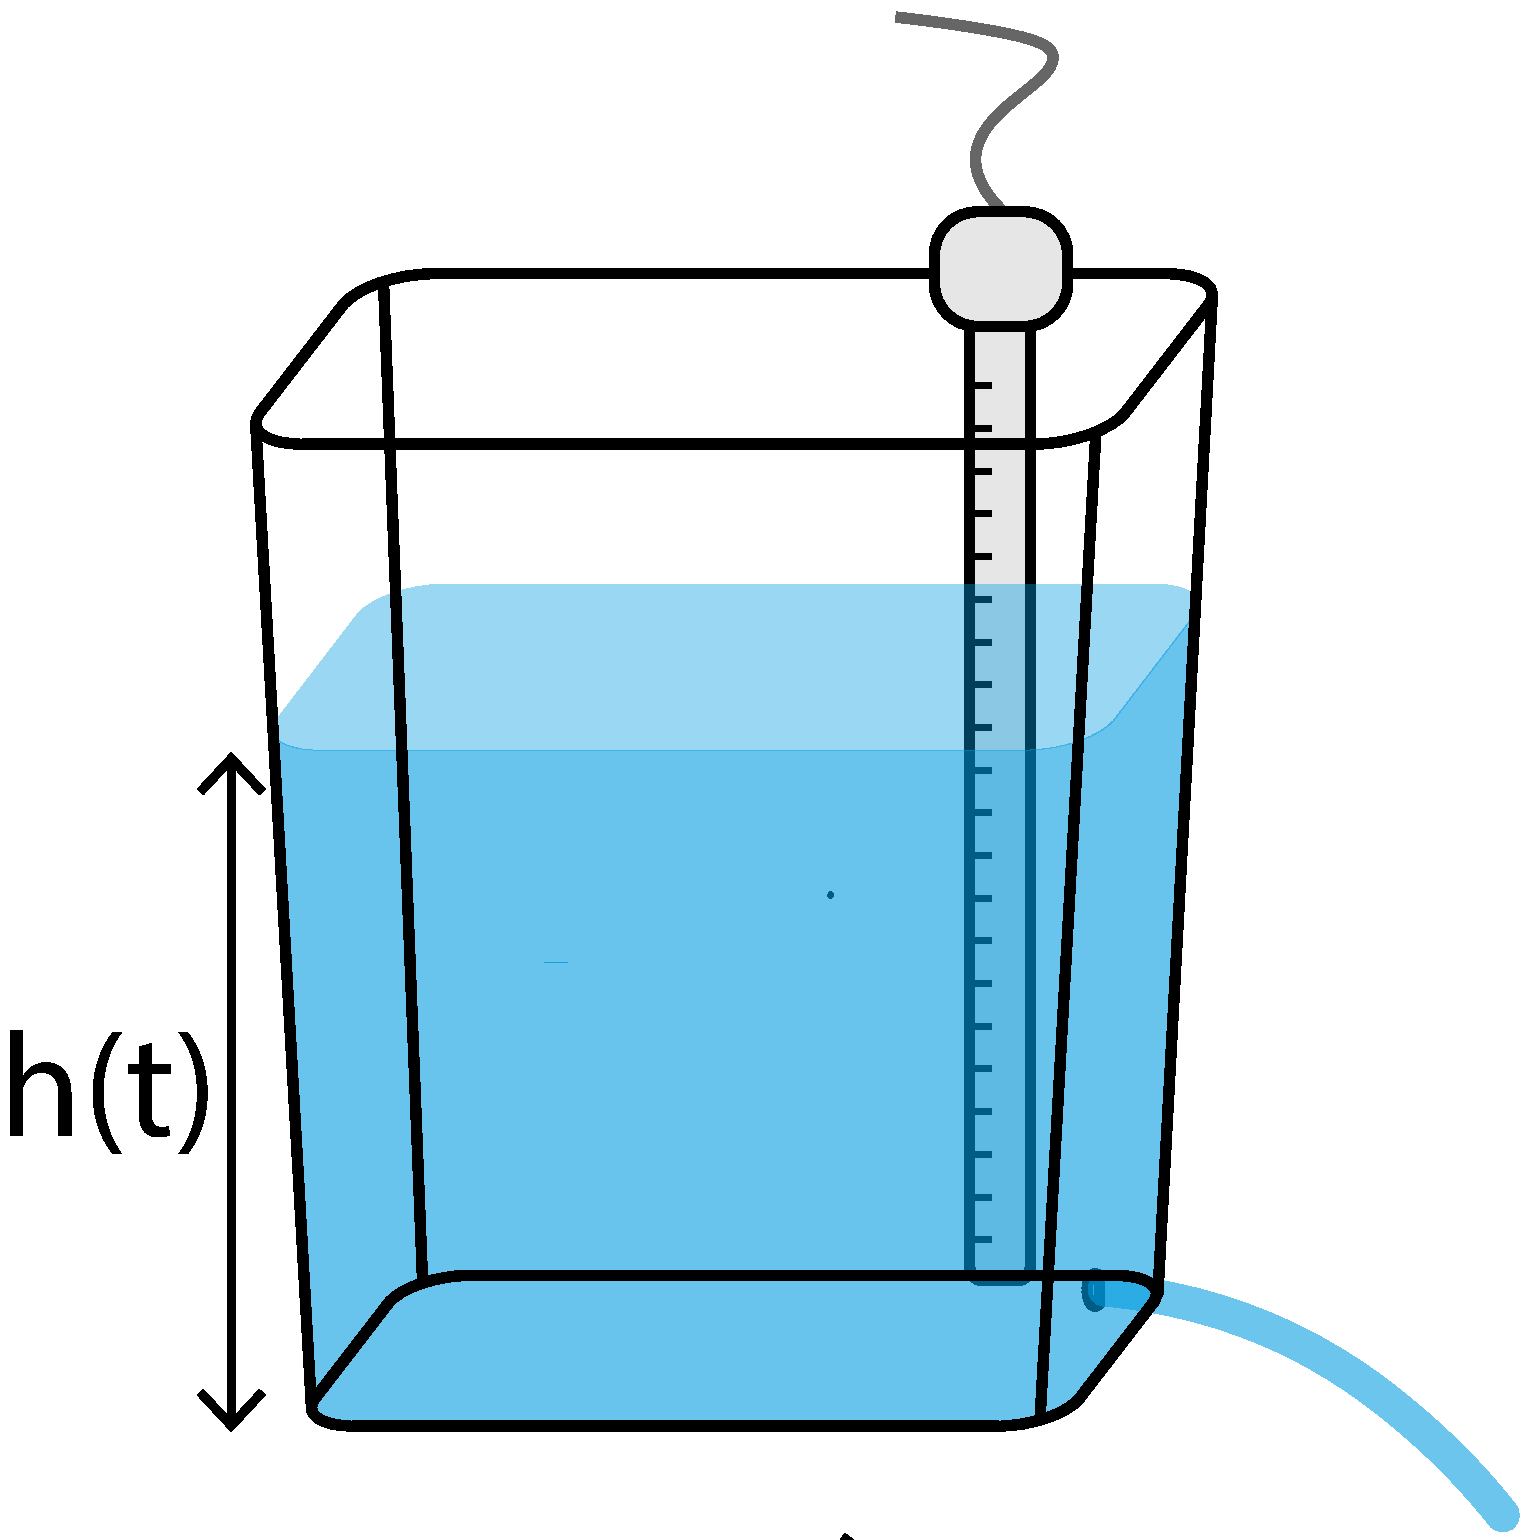
\includegraphics[width=\textwidth]{../tank_geometry/naked_tank.pdf}
	\caption{Experimental setup} \label{fig:naked_tank}
    \end{subfigure}
    
     \begin{subfigure}[b]{0.49\textwidth}
    	\includegraphics[width=\textwidth]{../prior_train.pdf}
	\caption{Prior dist'n of $h(t)$} \label{fig:prior_train}
    \end{subfigure}
     \begin{subfigure}[b]{0.49\textwidth}
    	\includegraphics[width=\textwidth]{../posterior_train.pdf}
	\caption{Data $\{(t_i, h_i)\}$ and posterior dist'n of $h(t)$} \label{fig:posterior_train}
    \end{subfigure}
    
     \begin{subfigure}[b]{0.49\textwidth}
    	\includegraphics[width=\textwidth]{../test.pdf}
	\caption{Test} \label{fig:test}
    \end{subfigure}
    \caption{
      \textbf{Model calibration.}
      }
\end{figure}

\begin{figure}[h!]
    \centering
        \begin{subfigure}[b]{0.3\textwidth}
    	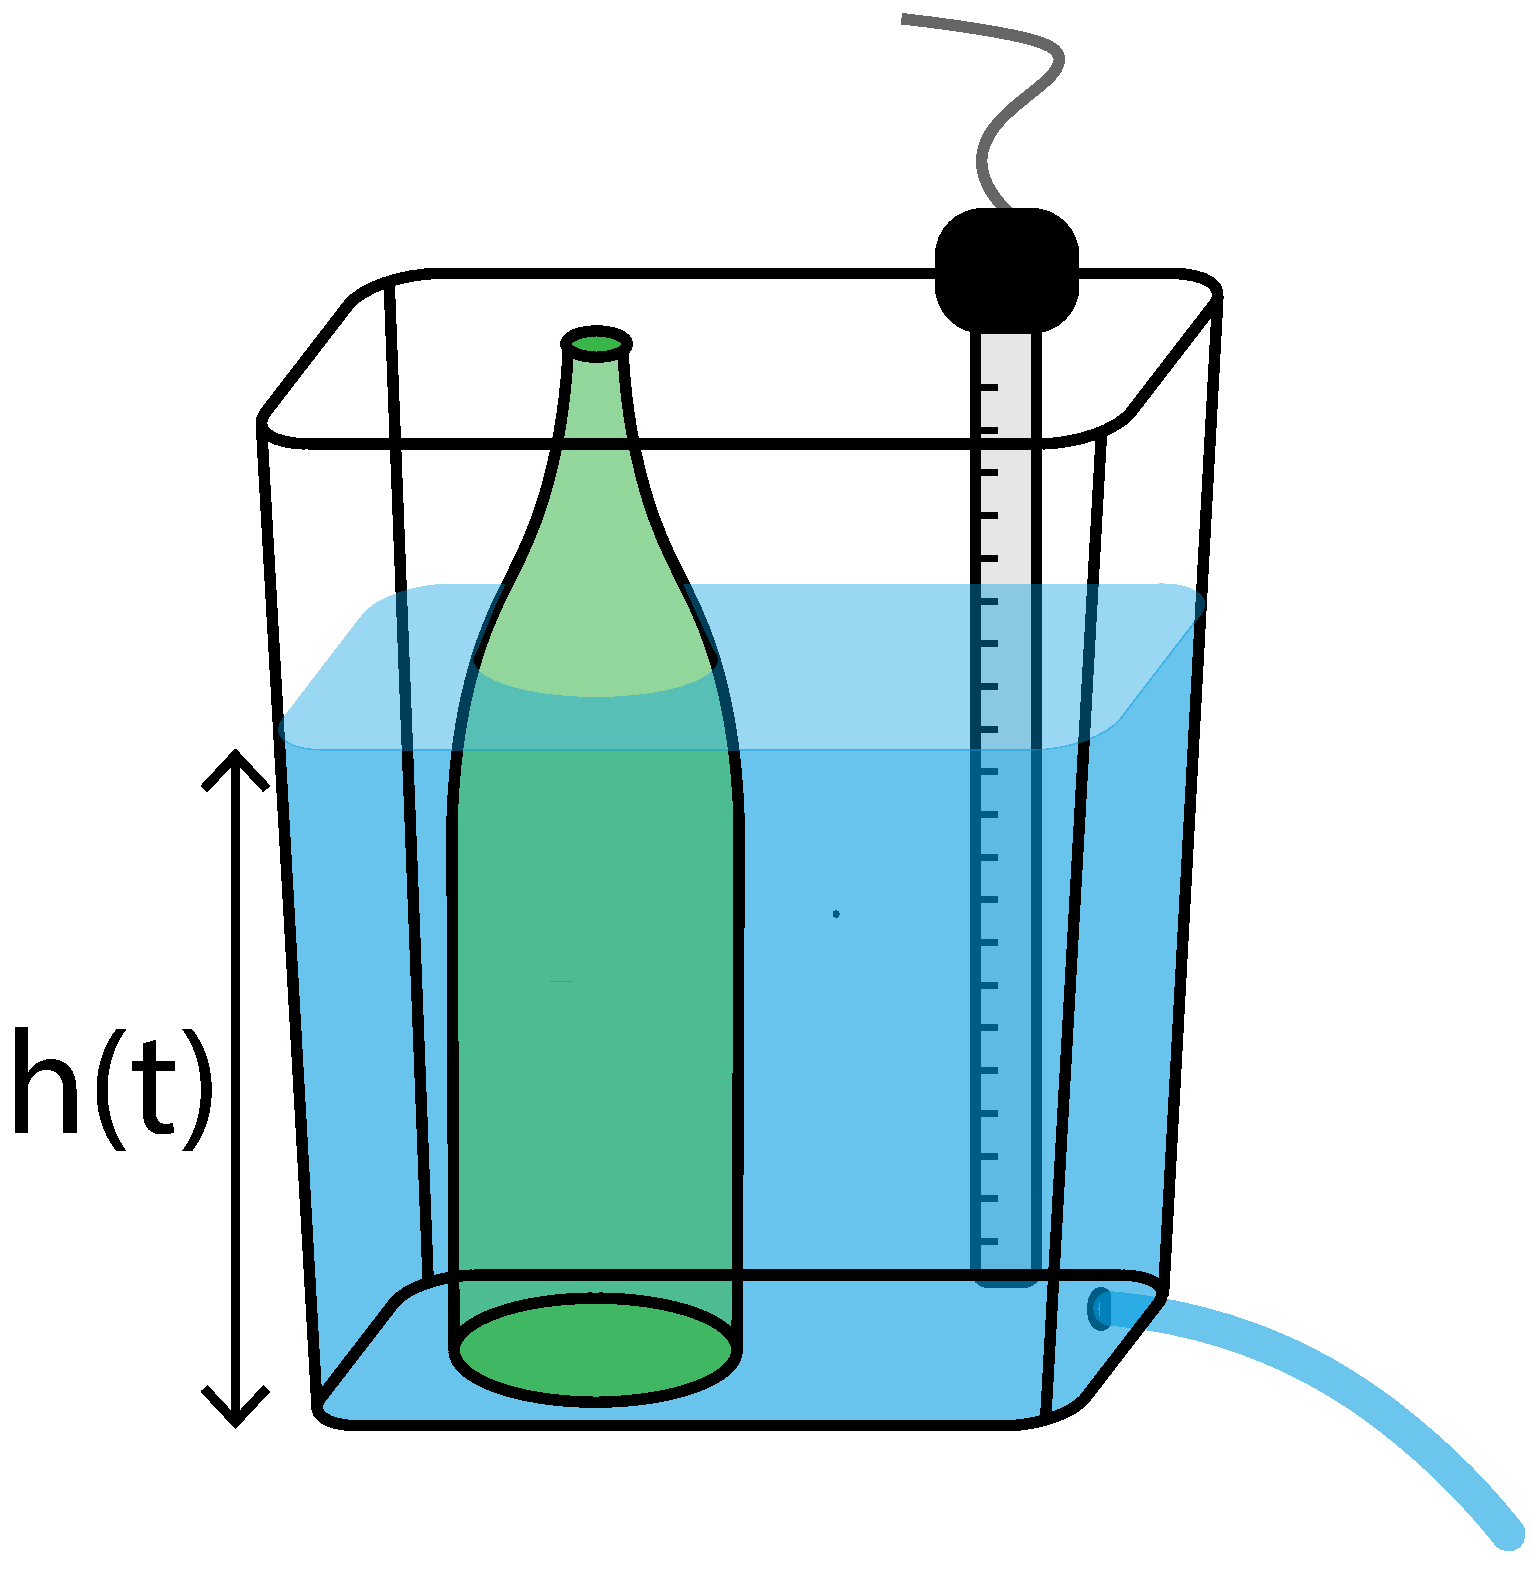
\includegraphics[width=\textwidth]{../tank_geometry/tank_w_bottle.pdf}
	\caption{Experimental setup} \label{fig:tank_w_bottle}
    \end{subfigure}
     \begin{subfigure}[b]{0.49\textwidth}
    	\includegraphics[width=\textwidth]{../posterior_object.pdf}
	\caption{Data $\{(t_i, h_i)\}$ and posterior dist'n of $h(t)$} \label{fig:posterior_object}
    \end{subfigure}
    
     \begin{subfigure}[b]{0.49\textwidth}
    	\includegraphics[width=\textwidth]{../prior_area.pdf}
	\caption{Prior dist'n of $a^\prime(h)$} \label{fig:prior_area.pdf}
    \end{subfigure}
       \begin{subfigure}[b]{0.49\textwidth}
    	\includegraphics[width=\textwidth]{../posterior_area.pdf}
	\caption{Posterior dist'n of $a^\prime(h)$} \label{fig:posterior_area.pdf}
    \end{subfigure}
    
  
    \caption{
      \textbf{Inferring the shape of the object in the tank.}
      }
\end{figure}

\section{Discussion}

Rocks inside tank. infer type of rock, coupled with packing. Popcorn polymer.

Surface tension dominates keeping the liquid from exiting. Then Torricelli's law not valid. Liquid stops emptyhing slightly above the hole. 

Mariotte's bottle \cite{kirevs2006mariotte}

\enlargethispage{20pt}

\ack{GF acknowledges ARMI for funding.}


%%%%%%%%%% Insert bibliography here %%%%%%%%%%%%%%

\vskip2pc


\bibliographystyle{RS} %%%% .BST file

\bibliography{refs} %%%%% .Bib file

\end{document}
